\documentclass[12 pt, twoside] {article}
\usepackage[margin=1in]{geometry}
\usepackage[utf8]{inputenc}
\usepackage{listings}
\usepackage{color}
\usepackage{textcomp}
\usepackage{setspace}
\usepackage{verbatim}
\usepackage{graphicx}
\usepackage{footnote}
\usepackage{enumitem}
\usepackage{fancyhdr}
\usepackage[parfill]{parskip}

\makesavenoteenv{tabular}
\makesavenoteenv{table}

\setlist[itemize]{noitemsep, topsep=0pt}

\newcommand\la{\textlangle}
\newcommand\ra{\textrangle}

\setlength{\parindent}{0pt}

\definecolor{codegreen}{rgb}{0,0.6,0}
\definecolor{codegray}{rgb}{0.5,0.5,0.5}
\definecolor{codeblue}{rgb}{0,0,0.6}
\definecolor{backcolor}{rgb}{0.95,0.95,0.95}

\lstdefinestyle{mystyle}{
	backgroundcolor = \color{backcolor},
	commentstyle = \color{codeblue},
	keywordstyle = \color{codegreen},
	numberstyle = \color{codegray},
	stringstyle = \color{magenta},
	basicstyle = \footnotesize\ttfamily,
	breakatwhitespace = false,
	breaklines = true,
	captionpos = b,
	keepspaces = true,
	numbers = left,
	numbersep = 5pt,
	showspaces = false,
	showstringspaces = false,
	showtabs = false,
	tabsize = 4
}

\lstset{style = mystyle}

\pagestyle{fancy}
\fancyhf{}
\rhead{Yicheng Wang}
\lhead{Trie}

\begin{document}
{\catcode`?=\active
\def?!#1!{\footnote{#1}}
\section*{Trie}

\subsection*{Definition}

A trie, or prefix tree, is a special data structure that functions as a
collection of strings (or any type of sequence where the absolute location in
the sequence matters). Before we dive into the applications and advantages of
using this data structure over others, let us first see what it is. (from this
point on, I will talk about trie in the context of storing a list of strings,
but similar concept can be applied to all type of sequential data structures)

A trie is a tree where each node holds one character. Each vertex is an
\textbf{associative prefix} to each of its child nodes. The tree is rooted at
the empty string, which is the universal prefix of the dictionary.

Pictorially a dictionary containing ``also,'' ``all,'' ``algo,'' ``assoc,''
``tree,'' ``trie,'' ``task,'' ``tasks,'' ``tank'' looks like:
\begin{figure}[h]
    \centering
    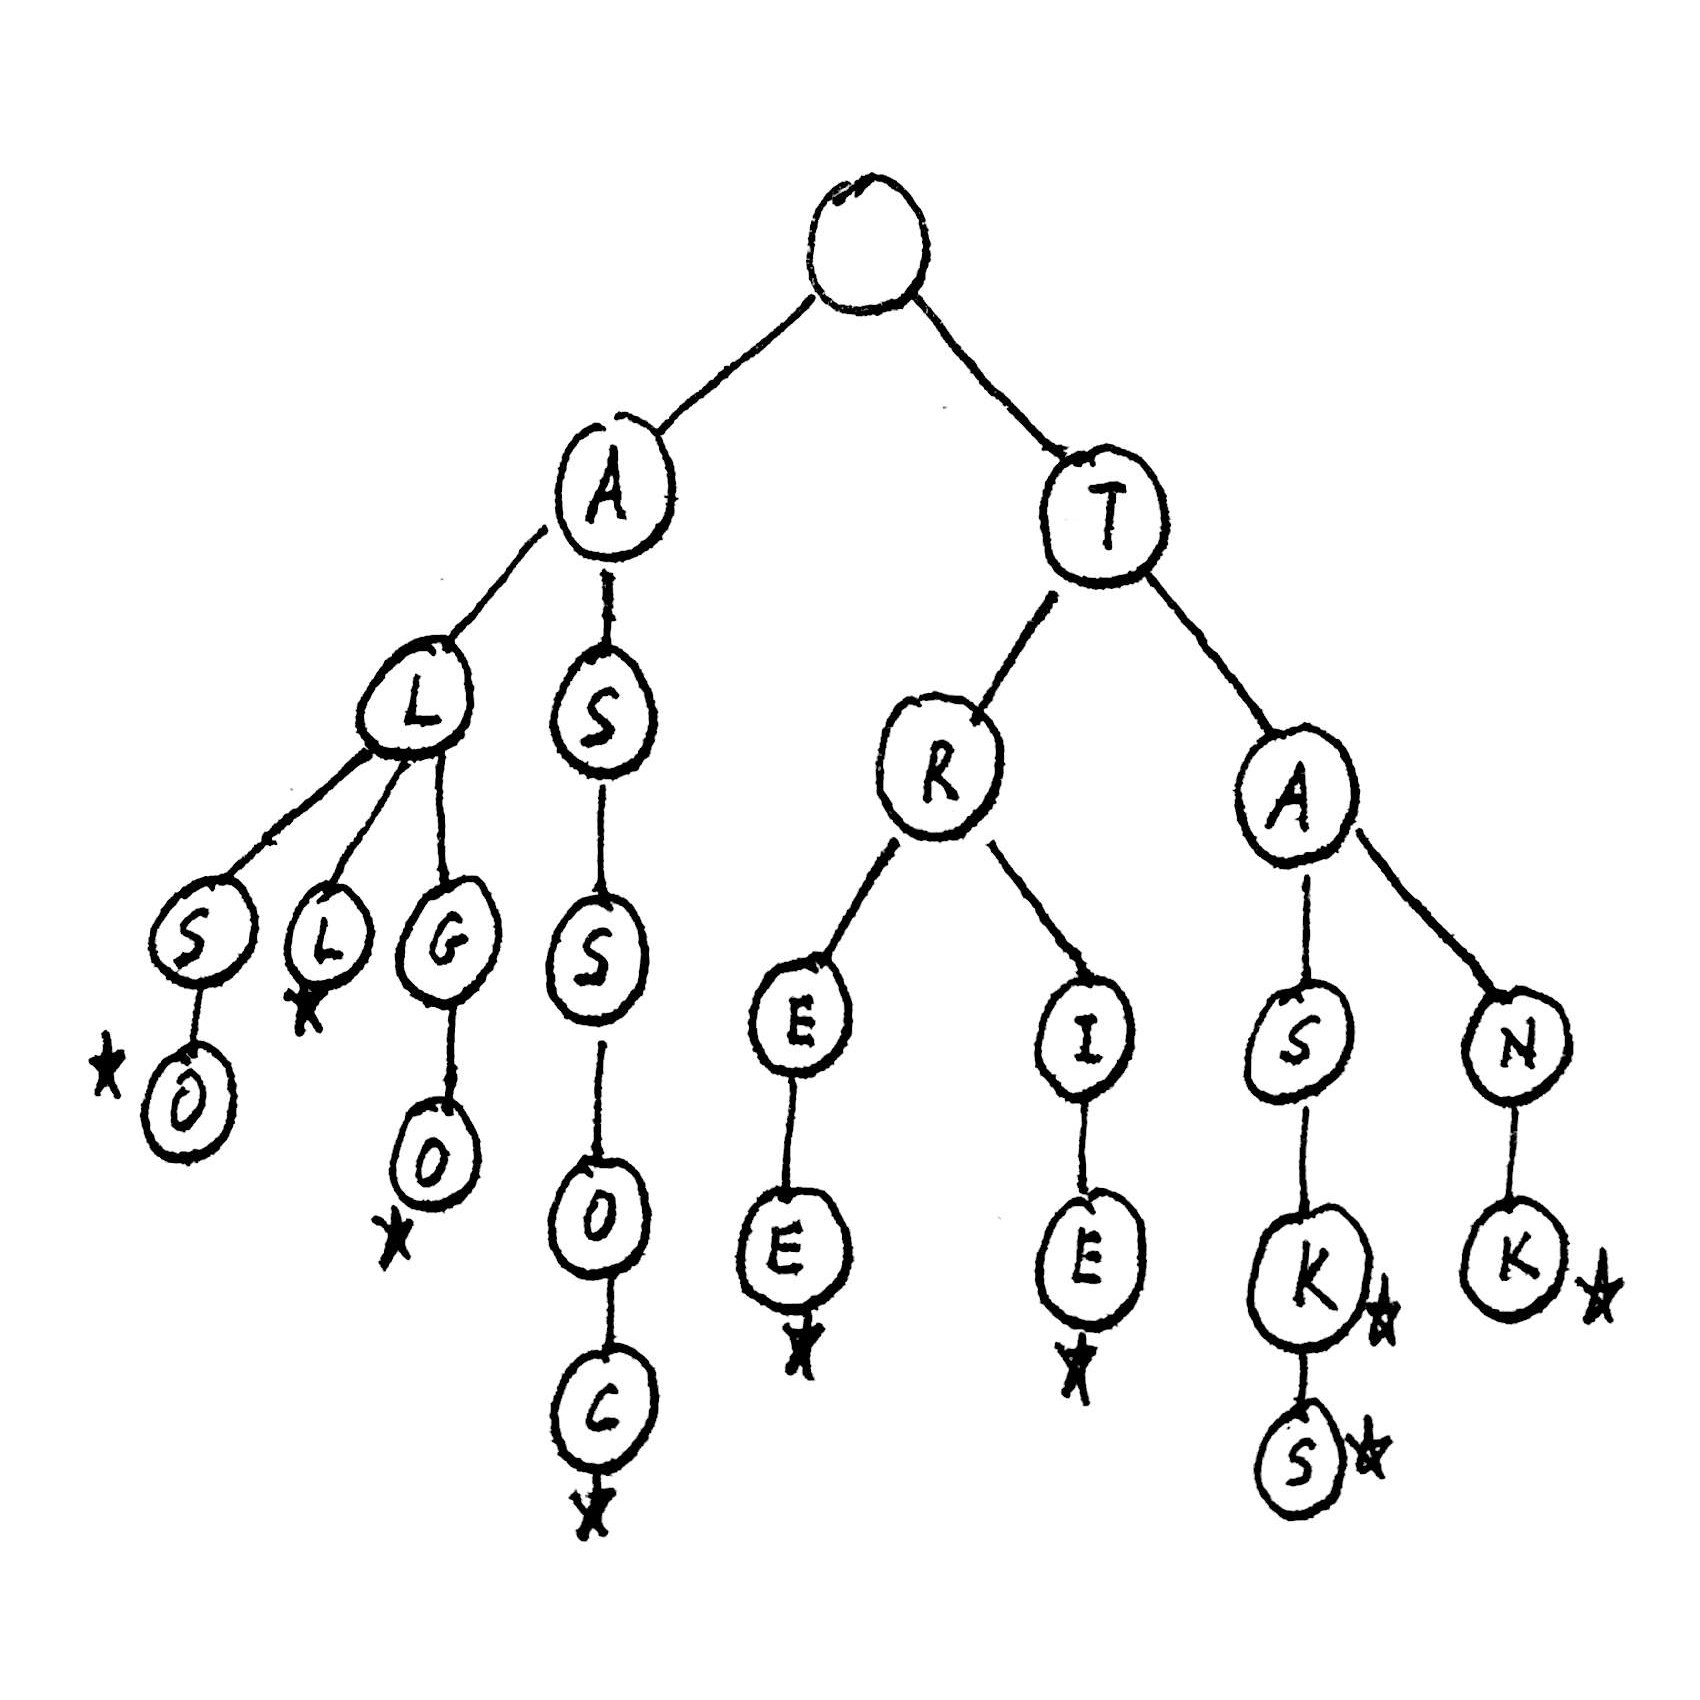
\includegraphics[width=0.4\textwidth]{trie.jpg}
\end{figure}

Note that the end of words are marked by a star, and note that ``task'' is
completed contained in the branch of ``tasks.'' This highlights one advantage of
using tries (not an important one, but pretty neat) which is that it offers some
degree of compression for a dictionary of strings where a lot of strings are
similar.

Note that another thing tries are amazing at and commonly used for is that it
can query which strings in a dictionary have a common prefix, as if they have a
common prefix, that prefix must be their common ancestor in the tree.

\subsection*{Operations and Implementation}

\subsubsection*{Node}

A node fundamentally need only 2 things, how many words terminate on this node
(can be replaced by a boolean if repeated words are not allowed), and a list of
references to its children. If this trie is used in a prefix-query heavy
context, one can also store how many words have the current node as a common
prefix. In code the structure should have the following fields:

\begin{lstlisting}[language=Java]
class TrieNode {
    int wordCount;
    int prefixCount;
    Map<Character, TrieNode> children;
}
\end{lstlisting}

\subsubsection*{Insert}

Insertion can be repeated until the string becomes the empty string:

\begin{lstlisting}[language=Java]
    void insert(String s) {
        if (s.length == 0) {
            wordCount++;
            prefixCount++;
            return;
        }

        char head = s.charAt(0);

        if (!children.containsKey(head)) {
            children.put(head, new TrieNode(0, 0, new HashMap<Character, TrieNode>()));
        }

        children.get(head).insert(s.substring(1));

        prefixCount++;
    }
\end{lstlisting}

This operation have runtime $O(L)$ where $L$ is the length of the string.

\subsubsection*{Contains}

To check if a word is in the dictionary we similarly repeatedly ask until
\texttt{s} becomes an empty string:

\begin{lstlisting}[language=Java]
    boolean contains(String s) {
        if (s.length == 0) {
            return wordCount > 0; // else this is not a word
        }

        char head = s.charAt(0);

        if (!children.containsKey(head)) {
            return false;
        }

        return children.get(head).contains(s.substring(1));
    }
\end{lstlisting}

This operation have runtime $O(L)$ where $L$ is the length of the string. (Note
that this is $O(1)$ in terms of size of the trie)

\subsubsection*{Query Prefix}

To check how many words have a given prefix we simply advance to the node
representing the prefix and return its \texttt{prefixCount}:

\begin{lstlisting}[language=Java]
    int countPrefix(String prefix) {
        if (prefix.length == 0) {
            return prefixCount;
        }

        head = prefix.charAt(0);

        if (!children.containsKey(head)) {
            return 0; // prefix doesn't exist
        }

        return children.get(head).countPrefix(prefix.substring(1));
    }
\end{lstlisting}

This operation have runtime $O(L)$ where $L$ is the length of the prefix.

\subsection*{Variations}

There are a lot of modifications we can make to the trie data structure to make
it more versatile. To start we can turn trie into an \textbf{associative data
structure}, more commonly known as a map. If we were to turn it into a map we
would just need an extra field within each node to store its \texttt{content},
which may be null if this is not a key in the map. This offers $O(L)$ access
time where $L$ is the length of the key.

Tries can also be used on primitive data types in the form of a
\textbf{bitwise-trie}. It takes the primitive data type and treats them as a
bit-array. This produces effectively a cache-independent binary search tree that
is in fact highly optimized and parallelized.

Further, the implementation went over here uses recursion for most of the
operations. While this is more intuitive than the iterative approach it is
slower due to how imperative programming languages function. I will send out a
version of trie that uses iteration instead of recursion with the same
operations as well.

\end{document}
